\documentclass[14pt,a4paper]{scrartcl}
\usepackage{cmap}
\usepackage[utf8]{inputenc}
\usepackage[T1,T2A]{fontenc}
\usepackage[english,russian]{babel}
\usepackage{relsize}
\usepackage{graphicx}
\usepackage{subfigure}
\usepackage{mathtools}
\usepackage{amssymb}
\usepackage{float}
\usepackage{sidecap}
\usepackage{wrapfig}
\usepackage{caption}
\usepackage[table,xcdraw]{xcolor}
\usepackage{listings}
\begin{document}
	\begin{titlepage}
	\begin{center}
		\large
		МИНИСТЕРСТВО ОБРАЗОВАНИЯ И НАУКИ\\ РОССИЙСКОЙ ФЕДЕРАЦИИ
		
		\vspace{0.5cm}
		
		МГТУ им Н.Э.Баумана
		\vspace{0.25cm}
		
		Факультет ФН
		
		Кафедра вычислительной математики и математической физики
		\vfill
		
		
		Соколов Арсений Андреевич\\
		\vfill
		
		
		{\LARGE Домашнее задание №2 по математической статистике\\[2mm]
		}
		\bigskip
		
		3 курс, группа ФН11-53Б\\
		Вариант 9
	\end{center}
	\vfill
	
	\newlength{\ML}
	\settowidth{\ML}{«\underline{\hspace{0.7cm}}» \underline{\hspace{2cm}}}
	\hfill\begin{minipage}{0.4\textwidth}
		Преподаватель\\
		\underline{\hspace{3cm}} Т.\,В.~Облакова\\
		«\underline{\hspace{0.7cm}}» \underline{\hspace{1.71cm}} 2019 г.
	\end{minipage}%
	\bigskip
	
	
	\vfill
	
	\begin{center}
		Москва, 2019 г.
	\end{center}
\end{titlepage}

\section{Моделирование выборки из заданного закона распределения}

Смоделируем выборку из дискретного закона распределения. Получим ряд распределения, принимая во внимание, что наша случайная величина подчинена биномиальному закону распределения с плотностью:
\begin{equation*}
	B(n,p) = \left(\begin{array}{l}{n} \\ {k}\end{array}\right) p^{k}(1-p)^{n-k},
\end{equation*}
$p = 0.7$ -- вероятность успеха в одном испытании;\\
$n = 140$ -- объем выборки;\\
$k = 8$ -- число испытаний.

\begin{lstlisting}
> k <- 8
> p1 <- 0.7
> n <- 140
> 
> distr_series_table <- as.data.frame(rbind(c(0:k),
+            dbinom(c(0:k), k, p1)), 
+            row.names = c("Random Value", "Probability"))
> colnames(distr_series_table) <- c(0:k)
> sum(distr_series_table[2,])
[1] 1
\end{lstlisting}

\begin{equation*}
	\begin{bmatrix}{}
	Random \: Value & 0.000 & 1.000 & 2.000 & 3.000 & 4.000 & 5.000 & 6.000 & 7.000 & 8.000 \\ 
	Probability & 0.000 & 0.001 & 0.010 & 0.047 & 0.136 & 0.254 & 0.296 & 0.198 & 0.058 \\ 
	\end{bmatrix}
\end{equation*}
Причём:
\begin{equation*}
	\sum_{i = 0}^{k}P_i = \sum_{i = 0}^{8}P_i = 1
\end{equation*}

Для моделирования такой дискретной случайной величины разобьём отрезок $[0;1]$ на $k+1 = 8 + 1 = 9$ последовательных отрезков $\Delta_0, \Delta_1, \dots, \Delta_{k}$, длины которых равны соответствующим вероятностям $P_0, P_1, \dots, P_{k}$.

Тогда длины отрезков будут равными: $\Delta_0 = P_0 - 0$, $\qquad \Delta_1 = (P_0 + P_1) - P_0 = P_1$ $\qquad \dots$$\qquad \Delta_n = 1 - (P_0 + P_1 + \dots + P_{n-1}) = P_n$

Видно, что длина частичного интервала с индексом $i$ равна вероятности $Р$ с тем же индексом. Длина $\Delta_i = P_i$.

Процедура получения конца $i-$го частичного интервала называется кумулятивным суммированием.

Далее, генерируем случайную величину $R$, равномерно распределенную на интервале $[0;1]$. При попадании случайной величины $r_i$ в частичный интервал $\Delta_i$ случайная величина $X$ принимает значение $x_i$ с вероятностью $P_i$ согласно теореме:\\
\textbf{Теорема.} Если каждому случайному числу $r_i(0\leq r_i < 1)$, которое попало в интервал $\Delta_i$, поставить в соответствие возможное значение $x_i$, то разыгрываемая случайная величина будет иметь заданный закон распределения.

Добавим к нашей таблице распределения третью строчку, соответствующую координатам концов интервалов разбиения отрезка $[0;1]$:
\begin{lstlisting}
> distr_series_table <- rbind(distr_series_table,
+                             cumsum(dbinom(c(0:k), k, p1)))
> row.names(distr_series_table)[3] <- "Delta"
\end{lstlisting}

Имеем:
\begin{equation*}
	\begin{bmatrix}{}
	Random Value & 0.000 & 1.000 & 2.000 & 3.000 & 4.000 & 5.000 & 6.000 & 7.000 & 8.000 \\ 
	Probability & 0.000 & 0.001 & 0.010 & 0.047 & 0.136 & 0.254 & 0.296 & 0.198 & 0.058 \\ 
	Delta & 0.000 & 0.001 & 0.011 & 0.058 & 0.194 & 0.448 & 0.745 & 0.942 & 1.000 \\ 
	\end{bmatrix}
\end{equation*}

Сгенерируем программным путём $n = 140$ случайных чисел:
\begin{lstlisting}
> set.seed(1337)
> rand_unif <- runif(n, 0, 1)
> head(rand_unif)
[1] 0.576321 0.564742 0.073990 0.453865 0.373279 0.331317
\end{lstlisting}
При установке параметра, такого же, как в первой строчке вышеприведённого кода, случайные величины будут сгенерированы на любом компьютере в точности равными тем, что получены в данной работе.

Случайное число $r_i = 0.57632155$ принадлежит шестому частичному интервалу, поэтому разыгрываемая случайная  величина приняла возможное значение $x_6 = 6$. Аналогично получим остальные возможные значения дискретной случайной величины $X$:

\begin{lstlisting}[basicstyle=\small]
>y <- rand_unif #tmp var for decreasing code
> emp_sample <- ifelse(y < distr_series_table[3,2], 0, 
+  ifelse(y < distr_series_table[3,3] & y >= distr_series_table[3,3-1], 1, 
+  ifelse(y < distr_series_table[3,4] & y >= distr_series_table[3,4-1], 2, 
+  ifelse(y < distr_series_table[3,5] & y >= distr_series_table[3,5-1], 3, 
+  ifelse(y < distr_series_table[3,6] & y >= distr_series_table[3,6-1], 4,
+  ifelse(y < distr_series_table[3,7] & y >= distr_series_table[3,7-1], 5,
+  ifelse(y < distr_series_table[3,8] & y >= distr_series_table[3,8-1], 6,
+  ifelse(y < distr_series_table[3,9] & y >= distr_series_table[3,9-1], 7,
+  ifelse(y < distr_series_table[3,10] & y >= distr_series_table[3,10-1], 
+                                                            8,NA)))))))))
\end{lstlisting}

Итого, последовательность смоделированных возможных значений дискретной случайной величины $X$ такова:
\begin{lstlisting}
> emp_sample
[1] 6 6 4 6 5 5 8 5 5 4 8 8 7 4 8 3 8 7 5 5 7
[22] 6 3 4 6 8 7 7 6 8 7 4 6 5 7 6 8 7 5 5 6 7
[43] 6 6 5 4 5 5 3 5 8 6 6 5 7 5 4 6 6 6 7 5 7
[64] 7 4 4 8 6 5 6 5 7 5 4 6 5 4 5 6 6 8 7 3 4
[85] 6 7 6 6 5 8 7 6 6 6 6 5 6 5 5 8 6 6 7 7 5
[106] 4 4 4 5 6 7 4 2 4 6 4 6 6 7 6 4 7 6 6 7 4
[127] 6 7 7 6 7 6 7 5 8 6 5 5 4 5
\end{lstlisting}


\section{Статистический ряд. Эмпирическая функция распределения}
Запишем группированный статистический ряд:
\begin{lstlisting}
> stat_series <- as.data.frame(rbind(c(0:k), 
+        c(0, hist_tmp$counts), 
+       (c(0, hist_tmp$counts) / n) ), 
+       row.names = c("Simulated values", 
+                     "Frequencies", 
+                     "Relative frequencies"))
> colnames(stat_series) <- c(0:k)
\end{lstlisting}
Имеем:
\begin{equation*}
\resizebox{.98\hsize}{!}{$
	\begin{bmatrix}{}
	Simulated \: values & 0.000 & 1.000 & 2.000 & 3.000 & 4.000 & 5.000 & 6.000 & 7.000 & 8.000 \\ 
	Frequencies & 0.000 & 0.000 & 1.000 & 4.000 & 21.000 & 31.000 & 42.000 & 27.000 & 14.000 \\ 
	Relative \: frequencies & 0.000 & 0.000 & 0.007 & 0.029 & 0.150 & 0.221 & 0.300 & 0.193 & 0.100 \\ 
	\end{bmatrix}
$}
\end{equation*}

Здесь $Simulated \: values$ -- уникальные значения из выборки; $Frequencies$ -- частота значения, то есть количество исходов, в которых случайная величина приняла данное значение; $Relative \: frequencies$ -- относительная частота данного значения по отношению к общему объёму выборки. Очевидно, что:
\begin{equation*}
	\sum_{j = 0}^{k} Freq_j = n,
\end{equation*}

\begin{equation*}
	\sum_{j = 0}^{k} Rel\_freq_j = 1
\end{equation*}

Совокупность пар $(Sim\_val_i, Rel\_freq_i), \: i=(\overline{0, k})$ называют иногда \textit{эмпирическим законом распределения}, а вышеприведённую таблицу -- \textit{таблицей частот}.

\textit{Эмпирической функцией распределения}, соответствующей выборке $X = {x_1, \dots, x_n}$ называется функция:
\begin{equation*}
	F_n^* = \frac{1}{n} \sum_{i = 1}^{n} I(x_i < x) = \frac{1}{n} \nu_n(x),
\end{equation*} 
$I(A)$ -- индикатор множества $A$,\\
$\nu_n(x)$ -- число выборочных значений, не превосходящих $x$.
 
Эмпирическая функция распределения $F_n^{*}( x )$ служит статистическим аналогом (оценкой) неизвестной функции распределения $F(x)$, которую называют при этом \textit{теоретической}.

Построим эмпирический и теоретические функции распределения:
\begin{lstlisting}
> library(fitdistrplus)
> 
> theor_distr <- rbinom(n, k, p1)
> 
> png(filename = "../img/theor_ecdf.png", 
+     width = 1920, height = 1080,
+     pointsize = 24, res = 96 * 1.25)
> par(mar = c(4, 4, 2, 1), xaxs = "i", yaxs = "i")
> plot(ecdf(x = theor_distr), 
+      col = "black", lwd = 3, verticals = F, axes = F,
+      xlim = c(0,k+1), ylim = c(0,1.2),
+      xlab = "Value", ylab = "CDF", main = "Theoretical CDF")
> axis(1, c(1:k))
> axis(2, seq(0.0, 1.2, 0.2), las = 1)
> grid(nx = k+1, ny = 1.2 / 0.2)
> dev.off()
RStudioGD 
2 
> 
> 
> png(filename = "../img/emp_ecdf.png", 
+     width = 1920, height = 1080,
+     pointsize = 24, res = 96 * 1.25)
> par(mar = c(4, 4, 2, 1), xaxs = "i", yaxs = "i")
> plot(ecdf(emp_sample), 
+      col = "red", lwd = 3, verticals = F, axes = F,
+      xlim = c(0,k+1), ylim = c(0,1.2),
+      xlab = "Value", ylab = "CDF", main = "Emperical CDF")
> axis(1, c(1:k))
> axis(2, seq(0.0, 1.2, 0.2), las = 1)
> grid(nx = k+1, ny = 1.2 / 0.2)
> dev.off()
RStudioGD 
2 
> 
> png(filename = "../img/emp_and_theor_ecdf.png", 
+     width = 1920, height = 1080,
+     pointsize = 24, res = 96 * 1.25)
> par(mar = c(4, 4, 2, 1), xaxs = "i", yaxs = "i")
> plot(ecdf(emp_sample), 
+      col = "red", lwd = 3, verticals = T, axes = F,
+      xlim = c(0,k+1), ylim = c(0,1.2),
+      xlab = "Value", ylab = "CDF", 
+      main = "Theoretical and Emperical CDF")
> plot(ecdf(theor_distr), 
+      col = "black", lwd = 2, verticals = T, add = T)
> axis(1, c(1:k))
> axis(2, seq(0.0, 1.2, 0.2), las = 1)
> grid(nx = k+1, ny = 1.2 / 0.2)
> legend("bottomright", c("Theoretical", "Emperical"), 
+        lty=c(1,1), 
+        fill=c("black", "red"))
> dev.off()
RStudioGD 
2 
\end{lstlisting}
\pagebreak

\begin{figure}[h]
	\begin{minipage}[h]{0.5\linewidth}
		\center{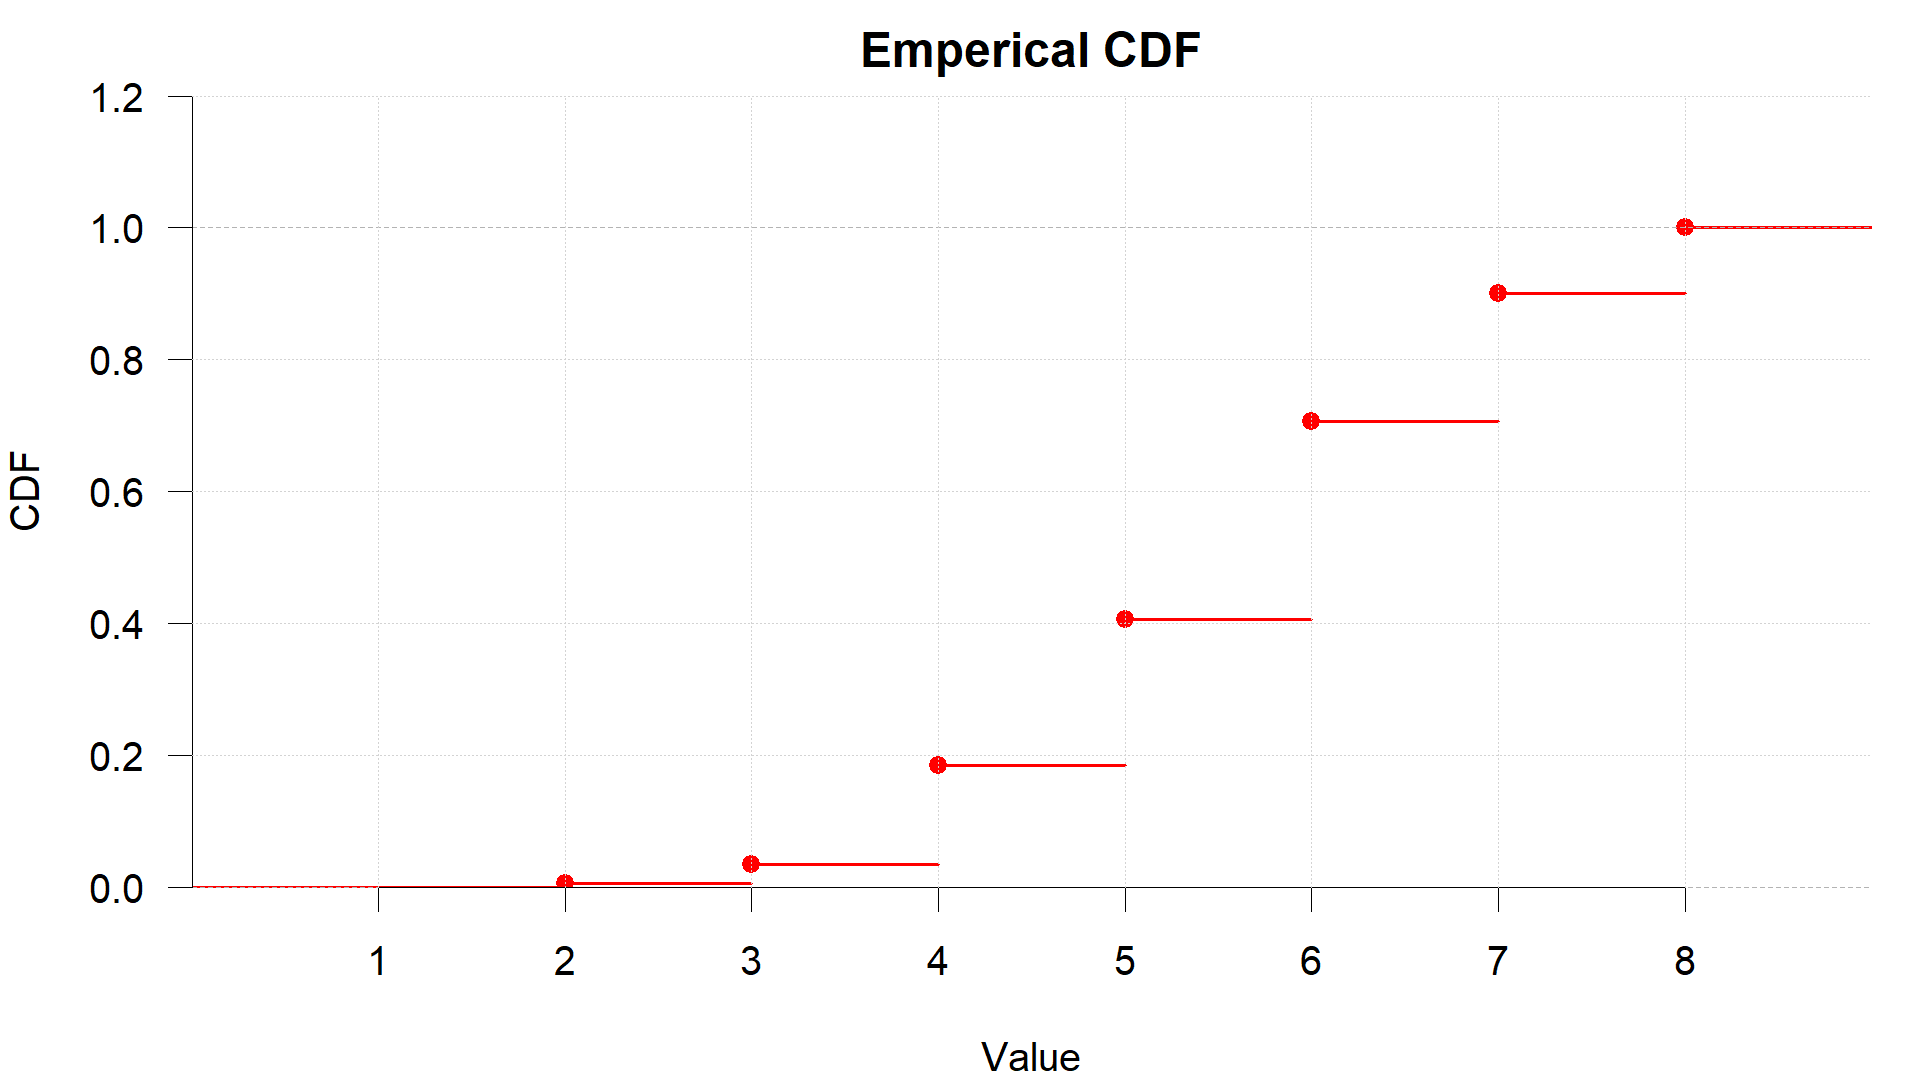
\includegraphics[width=0.9\linewidth]{../img/emp_ecdf.png}}
	\end{minipage}
	\hfill
	\begin{minipage}[h]{0.5\linewidth}
		\center{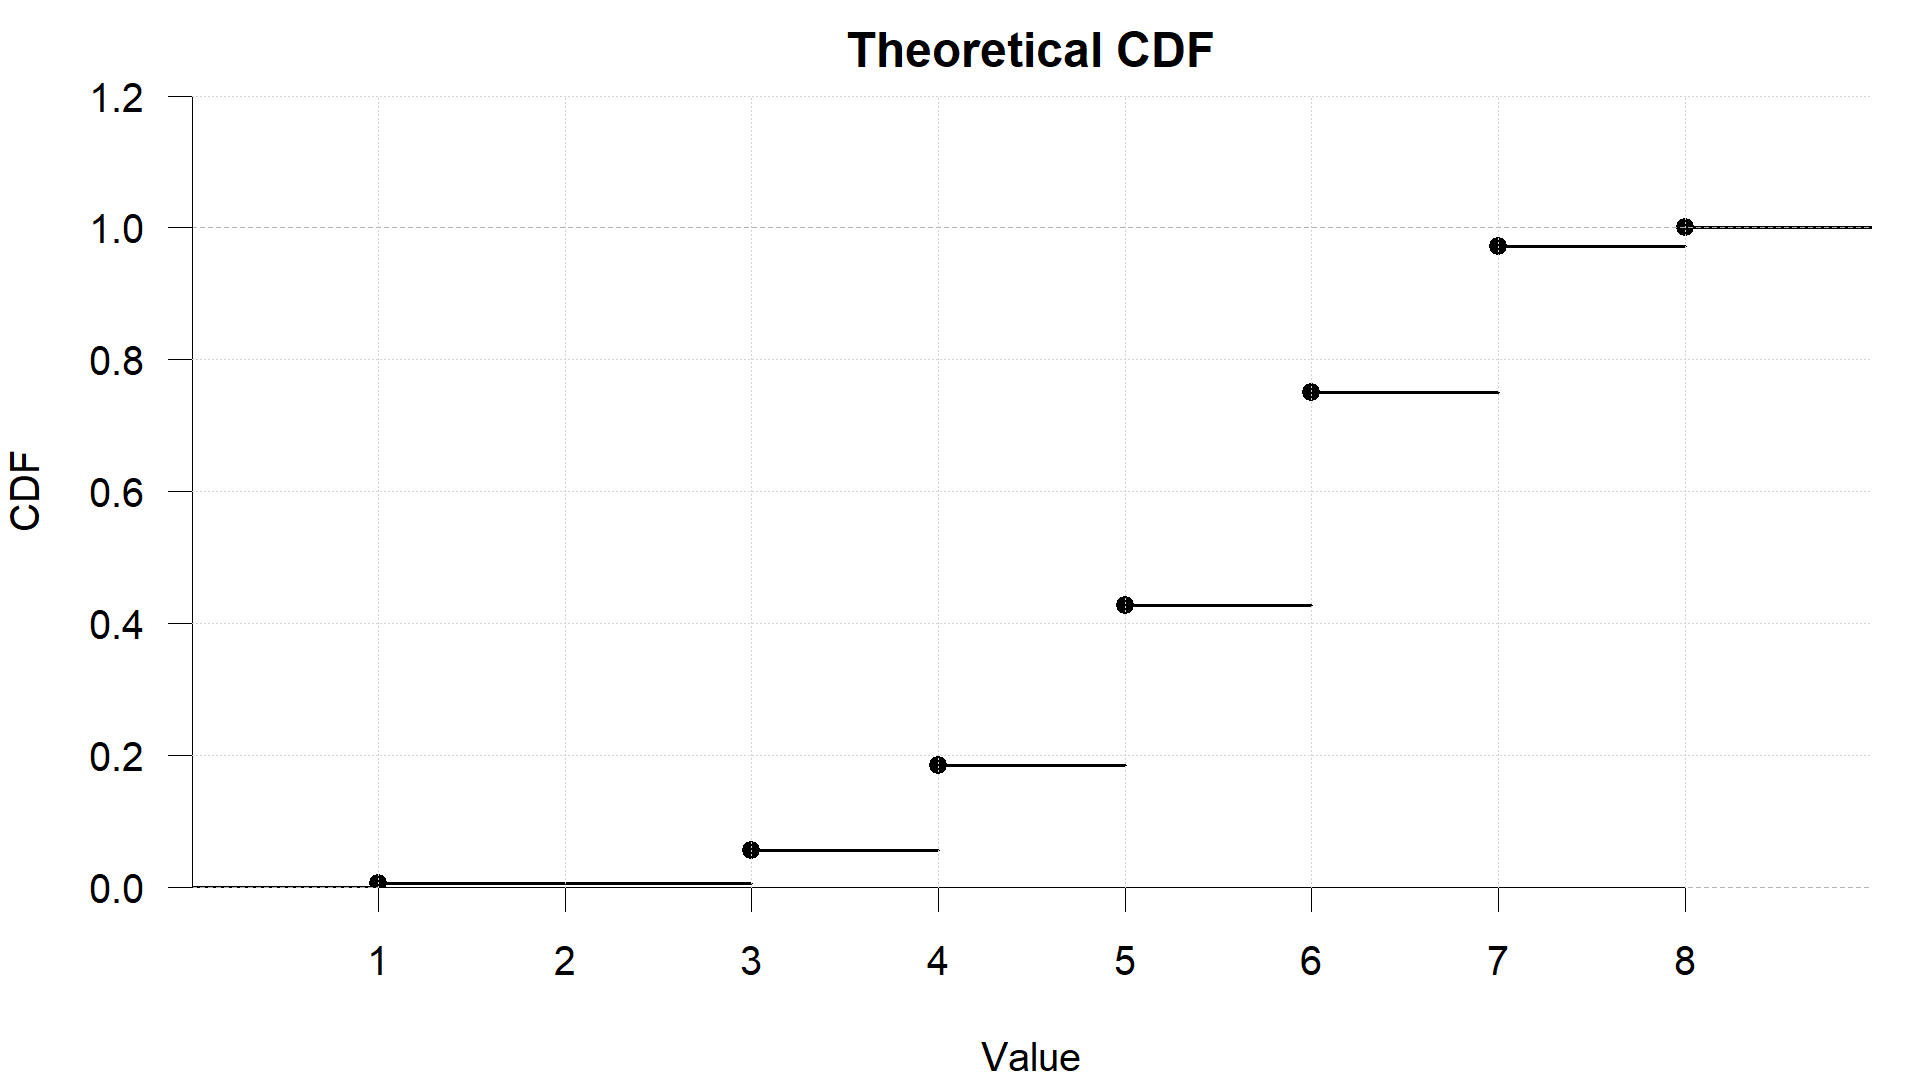
\includegraphics[width=0.9\linewidth]{../img/theor_ecdf.png}}
	\end{minipage}
	\label{ris:image1}
\end{figure}

\begin{figure}[h]
	\center{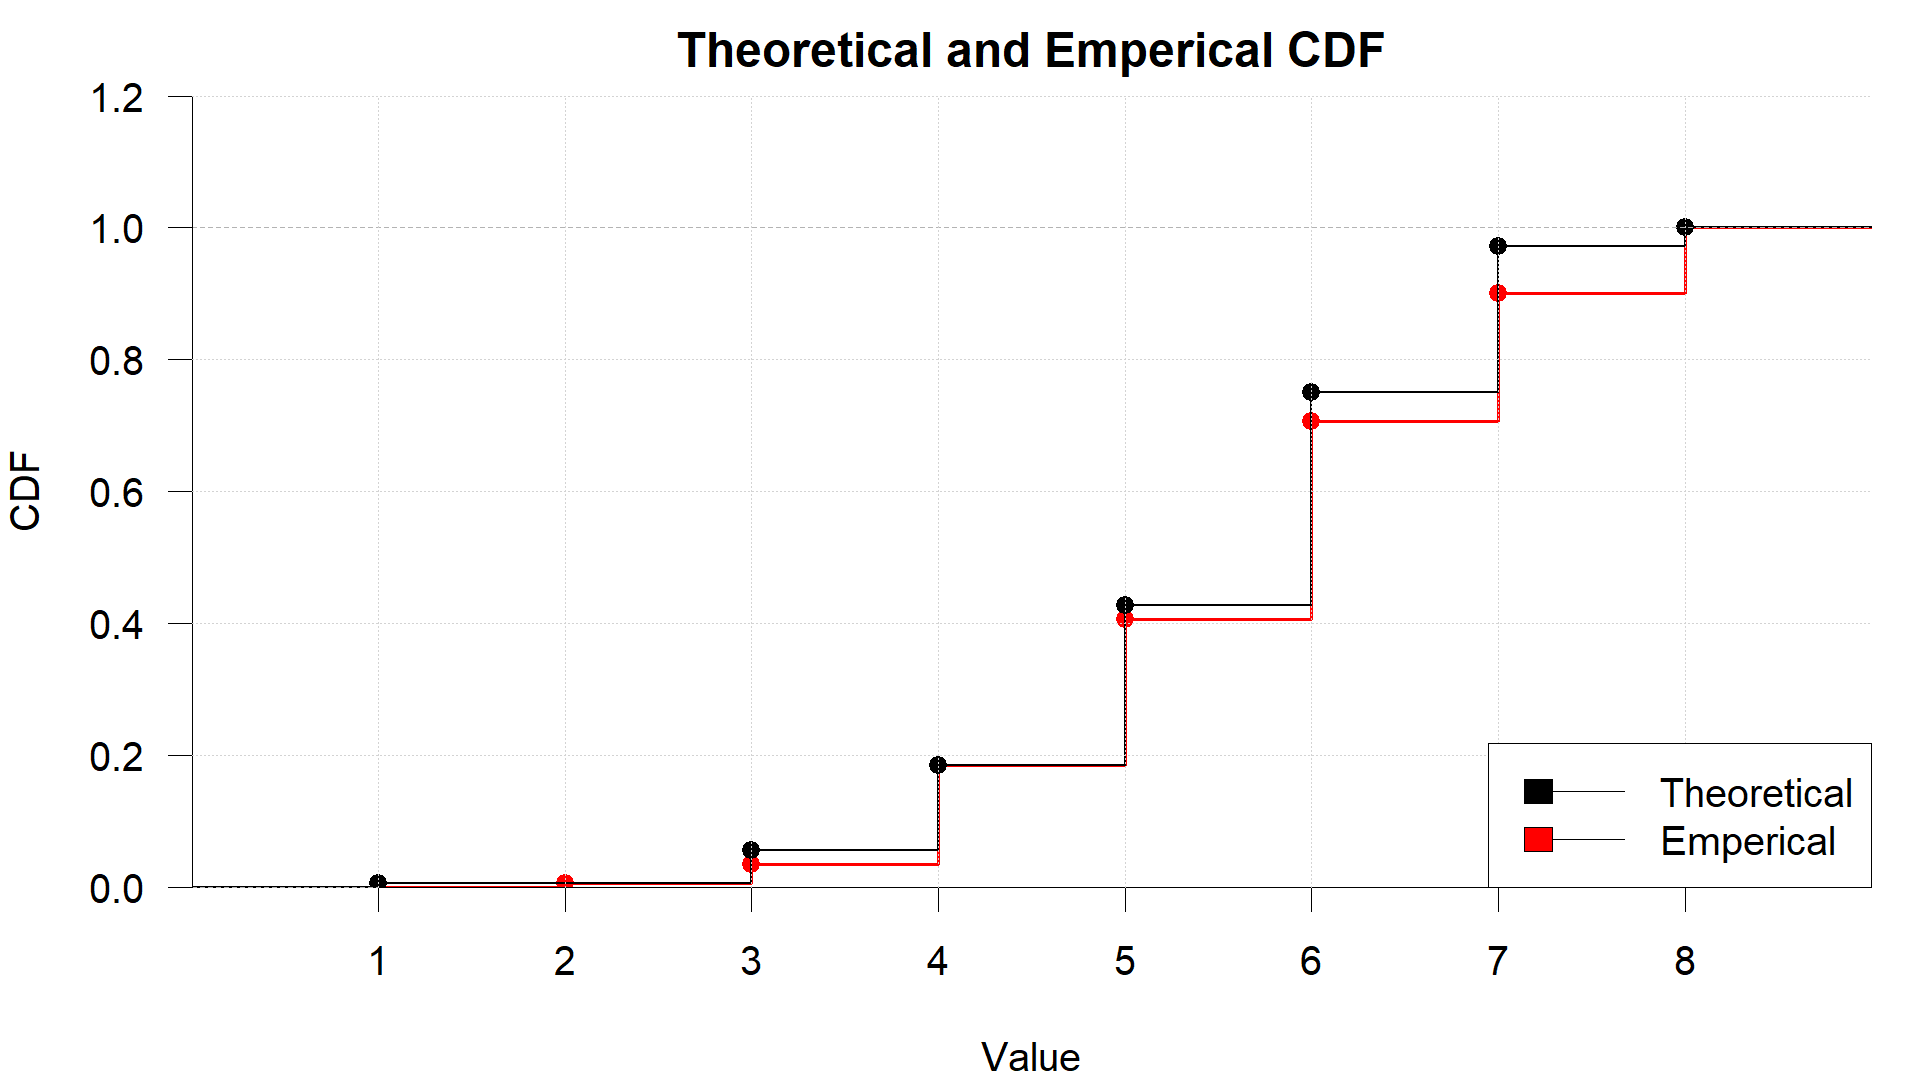
\includegraphics[width=1\linewidth]{../img/emp_and_theor_ecdf.png}}
	\label{ris:image}
\end{figure}

\section{Статистика Колмогорова. Меры}
Вычислим статистику Колмогорова для данного распределения по формуле:
\begin{equation*}
	D_{n}=\sup _{x}\left|F_{n}(x)-F(x)\right|
\end{equation*}

\begin{lstlisting}
> kolm_stat <- 
+    max(abs((cumsum(as.numeric(stat_series[3,]))
+    - pbinom(c(0:k), k, p1))))
> kolm_stat
[1] 0.04235199
\end{lstlisting}

Определим две меры для нашей выборки: стандартное отклонение и среднее:
\begin{lstlisting}
> theor_distr_mean <- mean(theor_distr)
> theor_distr_mean
[1] 5.464286
> 
> emp_sample_mean <- mean(emp_sample)
> emp_sample_mean
[1] 5.757143
> 
> 
> theor_distr_sd <- sd(theor_distr)
> theor_distr_sd
[1] 1.32171
> 
> emp_sample_sd <- sd(emp_sample)
> emp_sample_sd
[1] 1.318771
\end{lstlisting}








\end{document}